One realization of the continuous-time Markov chain for 5 years is illustrated in figure \ref{1realiz5yr}.
\begin{figure}
    \centering
    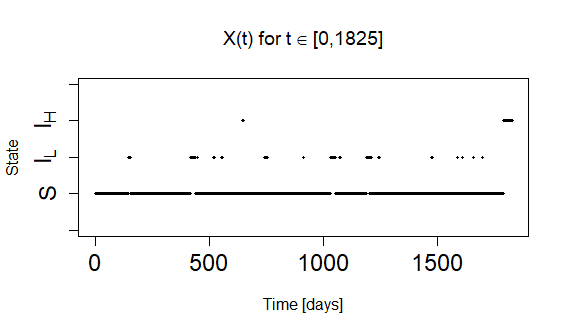
\includegraphics[width=130mm]{1real5yr.png}
    \caption{One realization of the continuous-time Markov chain $\{X(t):t \in [0, 1825]\}$.}
    \label{1realiz5yr}
\end{figure}
One can not tell much about the generally tendencies from this single realization. However, this realization shows that the individual will experience two heavy infections and some light infections within five years. It seems like the proportion of days in each state is corresponding well to the previous result stating that an individual is susceptible $92.33\%$, lightly infected $5.82\%$ and heavily infected $1.85\%$ of the time. 

%.... By calculating the mean time between infections one see that an individual will on average get a light cold every 100... days...and heavily infections once in 2.9 years.... . Har ikke regna ut dette i forgående oppgaver, 

